% Chapter 6

\chapter{RESULTS AND DISCUSSION} % Write in your own chapter title

\section{Results}
\subsection{Assessment}


\begin{figure}[H]
  \centering
  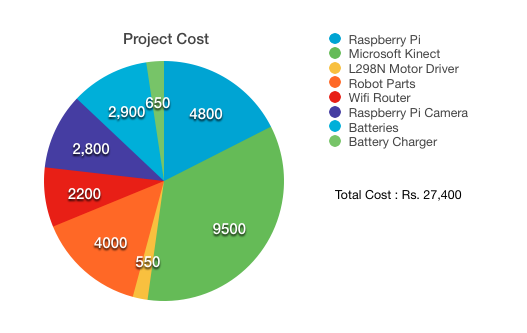
\includegraphics[width = 15cm, height = 9cm, scale=1]{graph4.png}
  \caption{Project Cost for each Part}
  \label{Cost wise Estimate}	
\end{figure}

\begin{table}[H]
    \begin{tabular}{ | l | l | l | p{2cm}|}
    \hline
    S.No & Test Case & Action & Result \\ \hline
    1 & SwipeRight & Swipe hand in the right direction & Robot moves in the right direction \\ \hline
    2 & SwipeLeft &  Swipe hand in the left direction & Robot moves in the left direction \\ \hline
    3 & SwipeUp & Swipe hand in the upward direction & Robot moves in the forward direction \\ \hline
     4 & SwipeDown & Swipe hand in the downward direction & Robot moves in the backward direction \\ \hline
 5 & Circle & Swipe hand in a circular manner & Robot rotates \\ \hline
 6 & DiagonalSwipe & Swipe hand in a diagonal manner & Robot does not move \\ \hline
 7 & Left handed gesture & Any gesture made with the left hand & Robot does not move \\ \hline


    \end{tabular}
\caption{Test Cases and Results}
\label{APT}
\end{table}

\subsection{Evaluation}
There are several differences between the Internet-based re- mote control systems and other tele-operating systems. Most of the tele-operating systems are based on private media, by which the transmission delay and data loss rate can be well modelled. The Internet in contrast is a public and shared resource in which various end users transmit data via the complex network simultaneously. The route for data transmission between two end points in a wide area is not fixed for different trials and the collision may be caused when two or more users transmit data via the same route simultaneously. Therefore the transmission efficiency of the Internet is difficult to be modelled at any time period.

\begin{figure}[H]
  \centering
  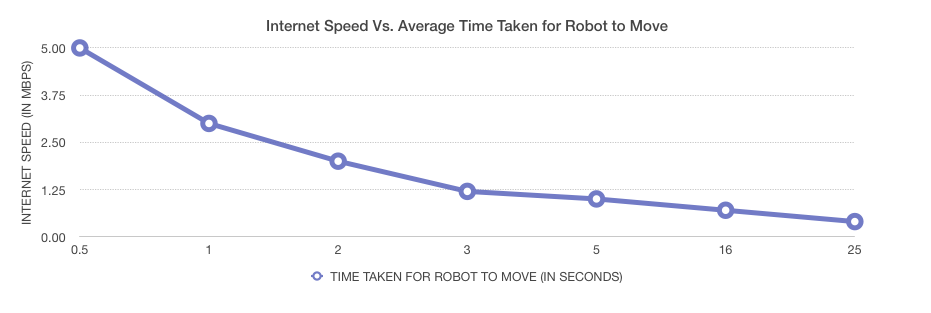
\includegraphics[width = 15cm, height = 7cm]{graph2.png}
  \caption{Time taken for Robot to Move based on Internet Speed}
  \label{Internet speed based performance}	
\end{figure}


\begin{figure}[H]
  \centering
  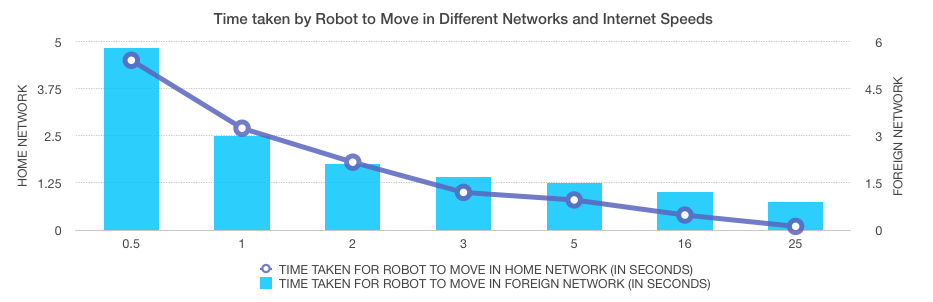
\includegraphics[width = 15cm, height = 6cm]{graph1.png}
  \caption{Time taken for Robot to Move in Different Networks based on Internet Speed}
  \label{Network based performance}	
\end{figure}

\begin{figure}[H]
  \centering
  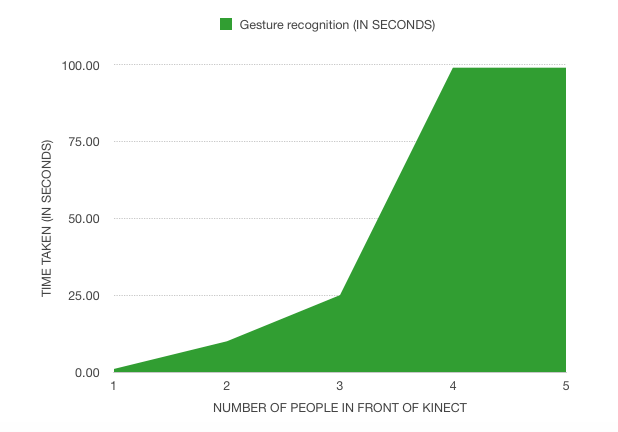
\includegraphics[width = 15cm, height = 11cm]{graph3.png}
  \caption{Time taken to Recognise Gesture based on Number of People in Front of Kinect}
  \label{Kinect performance}	
\end{figure}


\begin{figure}[H]
  \centering
  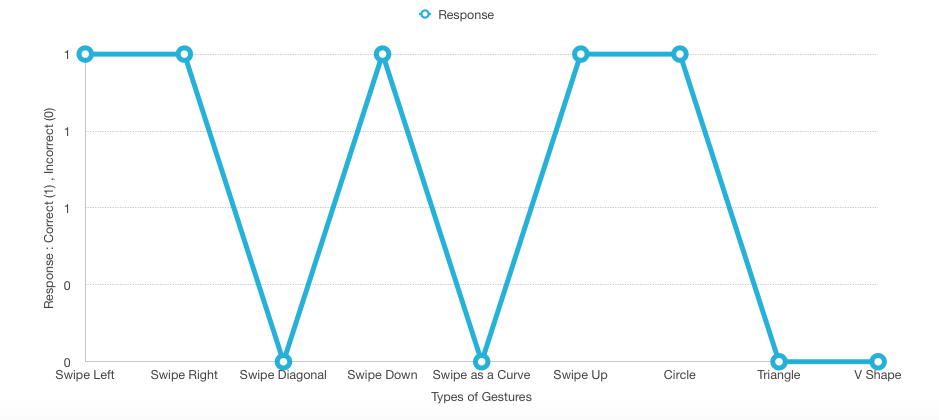
\includegraphics[width = 15cm, height = 7cm]{graph5.png}
  \caption{Response based on type of gesture}
  \label{Gesture-action pair}	
\end{figure}


